% Copyright 2026 Sreeram Anil
% SPDX-License-Identifier: CC-BY-4.0
% =============================================================================
%  High-gain observer
% =============================================================================
\chapter{High-Gain Observer with Anti-Peaking Saturation (HGO)}
\label{ch:hgo}

\section*{At a glance}
\begin{tabular}{@{}l>{\raggedright\arraybackslash}p{0.76\textwidth}@{}}
Family & Deterministic observers \\
Header & \texttt{include/estkit/observers/hgo.hpp} \\
Registered name & \texttt{HGO} \\
State dimension & $n_x = 4$ (cell model); $n_y = 1$ (static assertion) \\
Cost per step & $\mathcal{O}(n_x)$ steady state; $\approx 0.5\,\mu$s/step measured \\
Primary references & \cite{khalil2002,khalilpraly2014hgo,esfandiari1992saturation,khalil2017hgo} \\
\end{tabular}

\section{Motivation and aerospace/BMS relevance}
A high-gain observer is a Luenberger observer whose entire gain vector is parameterised by one
number.  In the observable canonical coordinates the gains scale as $\alpha_i/\varepsilon^i$, so
as $\varepsilon\to0$ the observer becomes arbitrarily fast and its estimate becomes arbitrarily
insensitive to bounded model uncertainty --- it reproduces the state of the true plant, not of
the model \cite{khalil2002,khalilpraly2014hgo}.  That is a strong property and it is why
high-gain observers underpin most output-feedback separation results for nonlinear systems.

It comes with an equally famous pathology: \emph{peaking}.  The transient response to an initial
error grows to $\mathcal{O}(\varepsilon^{-(n-1)})$ before decaying, which for $n=4$ and
$\varepsilon = 0.2$ is a factor of $125$.  In a feedback loop this can destabilise the plant; in
an estimator it drives the estimate far outside its physical range.  The standard remedy, due to
Esfandiari and Khalil \cite{esfandiari1992saturation}, is to saturate outside a compact set known
to contain the trajectory.

For a battery the attraction is the single knob.  A BMS integrator who wants ``recover from a
wrong initial SOC quickly, and I will accept the noise'' can turn $\varepsilon$ down; one who
wants a quiet estimate can turn it up.  Both directions are one number, and the anti-peaking
saturation makes the fast end safe, which is what makes this structure practical on a
safety-relevant estimate such as the reserve SOC of an eVTOL pack.

\section{Problem statement and assumptions}
Plant \eqref{eq:lue-plant-f}--\eqref{eq:lue-plant-h} with $n_y = 1$, $(\mA,\mC)$ observable, and
a bounded model uncertainty.  In addition,
\begin{assumption}[Known compact set]\label{as:hgo-compact}
A compact set containing the true state is known, and a per-state scale
$\varsigma_i>0$ is available such that a correction larger than $\mathcal{O}(\varsigma_i)$ per
sample is known to be spurious.
\end{assumption}
\Cref{as:hgo-compact} is exactly what the initial covariance $\mP_0$ handed to \texttt{init()}
encodes, and the implementation uses $\varsigma_i = \sqrt{\mP_{0,ii}}$.

\section{Derivation}

\subsection{Canonical form and the inverse-epsilon scaling}
For an observable single-output pair there exists $\bm{T}$ (built from the observability matrix
$\mathcal{O}$) such that $\bm{\xi} = \bm{T}\vx$ satisfies
\begin{equation}
\bm{\xi}_{k+1} = \mA_c\bm{\xi}_k + \bm{b}_c\,\varphi(\cdot) , \qquad y_k = \bm{c}_c\bm{\xi}_k ,
\label{eq:hgo-canon}
\end{equation}
with $(\mA_c,\bm{c}_c)$ in observer canonical (companion) form.  The high-gain observer takes
\begin{equation}
\mL_c = \Big[\ \frac{\alpha_1}{\varepsilon},\ \frac{\alpha_2}{\varepsilon^2},\ \dots,\
\frac{\alpha_n}{\varepsilon^{n}}\ \Big]^\T ,
\label{eq:hgo-gain}
\end{equation}
where $\alpha_i$ are the coefficients of a Hurwitz polynomial
$s^n + \alpha_1 s^{n-1} + \dots + \alpha_n$.  Substituting $\bm{\zeta}_i = \varepsilon^{\,n-i}
(\hat{\xi}_i-\xi_i)$ shows that the error dynamics in the $\bm{\zeta}$ coordinates are
independent of $\varepsilon$ up to a time scaling by $\varepsilon$: the observer is $1/\varepsilon$
times faster, and the uncertainty term is multiplied by $\varepsilon$ and therefore vanishes as
$\varepsilon\to0$ \cite[Sec.~14.5]{khalil2002}.  Peaking is the statement that the transformation
back, $\hat{\xi}_i - \xi_i = \varepsilon^{\,i-n}\zeta_i$, multiplies the transient by
$\varepsilon^{-(n-1)}$ in the first coordinate.

\subsection{Equivalent pole assignment}
The gain \eqref{eq:hgo-gain} is exactly what one obtains by placing the continuous-time observer
poles at $-\lambda_i/\varepsilon$, where the $\lambda_i$ are the roots of the nominal polynomial.
Discretising with sample time $\dt$,
\begin{equation}
p_i = \exp\!\left(-\frac{\lambda_i\,\omega_0\,\dt}{\varepsilon}\right)
     = \exp\!\left(-\frac{\lambda_i\,\mu}{\varepsilon}\right) ,
\qquad \mu \triangleq \omega_0\dt ,
\label{eq:hgo-poles}
\end{equation}
with $\omega_0$ the nominal ($\varepsilon=1$) bandwidth.  The implementation places
\eqref{eq:hgo-poles} directly in the \emph{original} coordinates with the shifted-and-scaled
Ackermann formula of \Cref{sec:lue-cond}.  This is not a cosmetic choice: for the 2-RC cell model
at $10$\,Hz, $\det\mathcal{O}\approx6\times10^{-18}$, so forming $\bm{T}$ from $\mathcal{O}$ and
inverting it --- the literal reading of \eqref{eq:hgo-canon} --- is numerically meaningless, while
Ackermann's formula needs only $\mathcal{O}\inv\bm{e}_n$ and, after the shift-and-scale, achieves
machine precision.

\subsection{Choice of the nominal roots}
The default is the \emph{binomial} observer, $\lambda_i = 1$ for all $i$, i.e. nominal polynomial
$(s+1)^n$ and $\alpha_i = \binom{n}{i}$ --- the textbook choice \cite[Ex.~14.7]{khalil2002}.  On
this plant it is also the only usable one, for the reason given in \Cref{sec:lue-spread}: three
of the four open-loop modes lie within $2\,\%$ of each other, and any spread $\{\lambda_i\}$ asks
for them to be pulled apart, which costs gains of order $10^2$--$10^3$ and a steady-state SOC
standard deviation of order $10^{-1}$.  With $\lambda_i\equiv1$ the closed-loop time constant is
simply
\begin{equation}
\tau_{cl} = \frac{\varepsilon}{\omega_0} ,
\label{eq:hgo-tau}
\end{equation}
which is the single design equation of the whole chapter.

\subsection{Anti-peaking saturation}
Following \cite{esfandiari1992saturation}, the correction is saturated componentwise outside the
compact set of \Cref{as:hgo-compact}:
\begin{equation}
\xplus_k = \xminus_k + \operatorname{sat}\!\big(\mL r_k;\ \bm{c}\big) ,
\qquad c_i = \varkappa\,\sqrt{\mP_{0,ii}} ,
\label{eq:hgo-sat}
\end{equation}
with $\varkappa = $ \texttt{Options::corr\_sigmas}.  Two remarks.  First, the saturation is on the
\emph{correction}, not on the innovation: saturating the innovation would also throttle the
legitimate large-residual transient, defeating the purpose.  Second,
$\mP_0$ is information the application already supplies through the estimator interface, so the
compact set is obtained without any model-specific constant.  \texttt{Model::constrain} is applied
afterwards and is the second projection, onto the physically feasible set.

How much the saturation is worth depends entirely on how large the gain underneath it is, and
this is where an earlier reading of this chapter has to be corrected.  With an \emph{uncertified}
pole-placement gain the saturation was the difference between $\mathrm{rmse}_{ss}=0.163$ (flagged
as diverged) and $0.009$ on \texttt{param\_mismatch}: it was rescuing a gain that should not have
been accepted in the first place.  Once every candidate gain is certified over the scheduling
family (\Cref{sec:lue-schedule}) the accepted gain is small, and disabling the saturation
($\varkappa\to\infty$) changes \texttt{param\_mismatch} and \texttt{nominal} not at all, and
\texttt{init\_error} and \texttt{combined} by about $4\,\%$ of whole-run rmse ($0.0395$ against
$0.0414$, and $0.0526$ against $0.0546$; three seeds).  The saturation is still the right thing to
implement --- it is what bounds the transient if the certification ever does admit a fast design,
and it costs two comparisons --- but on this plant, with a certified gain, it is a guard rail and
not a load-bearing member.  Two safety devices that overlap is the expected outcome; claiming
credit twice for the same failure is not.

\section{Algorithm}
\begin{algorithm}[H]
\caption{HGO --- one sampling period}
\begin{algorithmic}[1]
\Require $\xplus_{k-1}$, $\vu_{k-1}$, $y_k$, $\vu_k$, gain $\mL$, scales $\bm{\varsigma}=\sqrt{\diag\mP_0}$
\State \textbf{Time update:} $\xminus_k \gets f(\xplus_{k-1},\vu_{k-1})$; \quad $\hat{y}_k \gets h(\xminus_k,\vu_k)$
\If{the linearisation has moved by more than $\delta_{\mathrm{tol}}$}
  \State $p_i \gets \exp(-\lambda_i\mu/\varepsilon)$, $i=1..n_x$
  \State $\mL_{\mathrm{new}} \gets$ shifted-scaled Ackermann, converted with $\mA\inv$
  \State accept if $\norm{\mL_{\mathrm{new}}}_\infty\le L_{\max}$ and the robust check \eqref{eq:lue-robust} passes; LQE gain at start-up otherwise
\EndIf
\State $r_k \gets y_k-\hat{y}_k$; \quad $\Delta\vx \gets \mL r_k$
\For{$i = 1..n_x$} \State $\Delta x_i \gets \operatorname{clamp}(\Delta x_i,\ \pm\varkappa\varsigma_i)$ \Comment{anti-peaking} \EndFor
\State $\xplus_k \gets \operatorname{constrain}(\xminus_k + \Delta\vx)$
\Ensure $\xplus_k$
\end{algorithmic}
\end{algorithm}

\section{Application to the battery model}
Benchmark options: $\varepsilon = 0.2$, $\omega_0 = 1/300$\,s$^{-1}$ so that
$\tau_{cl} = \varepsilon/\omega_0 = 60$\,s by \eqref{eq:hgo-tau}, $\lambda_i\equiv1$,
$\varkappa = 0.5$, $L_{\max}=0.3$, and $q_{\text{extra},\soc}=10^{-4}$ for the start-up LQE
design.  With $\sqrt{\diag\mP_0} = [0.1,\ 2\,\mathrm{mV},\ 5\,\mathrm{mV},\ 0.5]$ the per-sample
correction limits are $[0.05,\ 1\,\mathrm{mV},\ 2.5\,\mathrm{mV},\ 0.25]$ --- generous enough to
allow a $35\,\%$ SOC error to be corrected in a handful of samples if the residual warranted it,
tight enough that a peaking transient cannot leave the physical range.

The measured $\varepsilon$ sweep on the eVTOL mission is the clearest available illustration of
the high-gain trade-off, and is reproduced here because it is the design curve a practitioner
would actually use:
\begin{center}
\begin{tabular}{@{}lrrrrr@{}}
\toprule
$\varepsilon$ & $\tau_{cl}$ [s] & nominal $\mathrm{rmse}_{ss}$ & \texttt{init\_error} conv [s]
 & \texttt{param\_mismatch} $\mathrm{rmse}_{ss}$ & \texttt{cold} \\
\midrule
$0.10$ & $30$ & $0.0018$ & $230$ & $0.0454$ & diverged \\
$0.15$ & $45$ & $0.0016$ & $296$ & $0.0271$ & ok \\
$0.20$ & $60$ & $0.0014$ & $408$ & $0.0169$ & ok \\
$0.30$ & $90$ & $0.0011$ & $101$ & $0.0087$ & ok \\
\bottomrule
\end{tabular}
\end{center}
The non-monotone convergence column is worth reading carefully: it is \emph{not} true here that
smaller $\varepsilon$ always converges faster, because below $\varepsilon\approx0.25$ an
increasing fraction of the scheduled re-designs is rejected by the gain budget and the observer
falls back on a slower validated gain.  The $\varepsilon=0.1$ row shows the genuine limit: at a
$30$\,s closed-loop time constant the gain required at low current is large enough that the
design is no longer robust to the scheduling and the \texttt{cold} scenario diverges.  For this
plant the usable range is $\varepsilon\gtrsim0.15$.

\section{Implementation notes}
$4672$ bytes and $0.5\,\mu$s/step.  There is no
covariance and, in steady state, no $\mathcal{O}(n_x^3)$ path; the $\mathcal{O}(n_x^3)$ design
runs only on a scheduling event.  The saturation adds $n_x$ comparisons.

Numerical points specific to this observer: the canonical transformation is \emph{never} formed
(see above); $\varepsilon$ is floored at $10^{-6}$ so that \eqref{eq:hgo-poles} cannot overflow;
the gain budget of \Cref{sec:lue-schedule} is what prevents the classic high-gain failure of a
design that is valid only at the linearisation point.  The float build reproduces the double
build to the printed precision, which would not be the case if the observability matrix were
inverted explicitly.

Limitation: the observer has no mechanism for a persistent output bias, so it inherits
\eqref{eq:lue-ssbias} in full.  Making $\varepsilon$ small does \emph{not} help against it, since
the equilibrium is gain-independent; it only makes the estimate track the time-varying part of
$\delta$ more faithfully, which is why the $\varepsilon$ sweep above shows
\texttt{param\_mismatch} getting \emph{worse} as $\varepsilon$ decreases.

\section{Benchmark results}
% Copyright 2026 Sreeram Anil
% SPDX-License-Identifier: CC-BY-4.0
\begin{table}[H]\centering\footnotesize\setlength{\tabcolsep}{4pt}
\caption{HGO: cell-level benchmark on the eVTOL mission (mean over seeds; RMSE and max error in \% SOC; $t_\mathrm{conv}$: first time the error stays below 2\,\% for 60\,s, -- = never; EKF reference: steady-state RMSE of the plain EKF on the same data).}\label{tab:cell_HGO}
\begin{tabular}{llrrrrrcrr}\toprule
plant & scenario & RMSE & RMSE$_\mathrm{ss}$ & max & $t_\mathrm{conv}$ [s] & RMSE$_v$ [mV] & div. & EKF ref. & ns/step \\ \midrule
ECM & nominal & 0.19 & 0.08 & 0.59 & 0 & 0.82 & no & 0.05 & 479 \\
ECM & init\_error & 3.93 & 0.07 & 33.70 & 329 & 5.63 & no & 0.05 & 528 \\
ECM & current\_bias & 0.87 & 0.85 & 1.67 & 0 & 0.86 & no & 0.61 & 475 \\
ECM & noise\_step & 0.32 & 0.33 & 1.16 & 0 & 3.22 & no & 0.12 & 2139 \\
ECM & outliers & 0.19 & 0.17 & 0.86 & 0 & 2.25 & no & 0.21 & 983 \\
ECM & cold & 1.60 & 0.40 & 6.26 & 0 & 2.47 & no & 0.16 & 367 \\
ECM & hot & 0.17 & 0.04 & 0.58 & 0 & 0.58 & no & 0.03 & 522 \\
ECM & aged\_cell & 2.22 & 2.18 & 6.03 & 0 & 3.44 & no & 1.52 & 651 \\
ECM & param\_mismatch & 1.31 & 1.49 & 5.30 & 0 & 2.69 & no & 1.36 & 548 \\
ECM & sensor\_dropout & 0.21 & 0.08 & 1.71 & 0 & 1.73 & no & 0.46 & 488 \\
ECM & preisach & 0.82 & 1.00 & 1.66 & 0 & 0.85 & no & 0.20 & 492 \\
ECM & combined & 5.25 & 2.11 & 24.28 & 804 & 7.19 & no & 12.44 & 458 \\
\midrule
SPM & nominal & 0.81 & 0.61 & 3.57 & 0 & 1.07 & no & 3.73 & 339 \\
SPM & init\_error & 5.60 & 1.86 & 33.71 & 1375 & 5.35 & no & 3.81 & 333 \\
SPM & current\_bias & 0.69 & 0.57 & 3.39 & 0 & 1.14 & no & 5.69 & 336 \\
SPM & noise\_step & 0.84 & 0.68 & 3.57 & 0 & 3.36 & no & 3.30 & 1149 \\
SPM & outliers & 0.83 & 0.60 & 4.10 & 0 & 2.39 & no & 1.99 & 589 \\
SPM & cold & 2.87 & 3.49 & 9.47 & 0 & 4.53 & no & 7.35 & 366 \\
SPM & hot & 0.76 & 0.61 & 4.40 & 0 & 0.75 & no & 2.16 & 342 \\
SPM & param\_mismatch & 1.81 & 1.27 & 5.51 & 0 & 1.90 & no & 3.13 & 322 \\
SPM & sensor\_dropout & 0.87 & 0.60 & 6.46 & 0 & 1.98 & no & 5.31 & 343 \\
\bottomrule\end{tabular}\end{table}

\begin{figure}[H]\centering
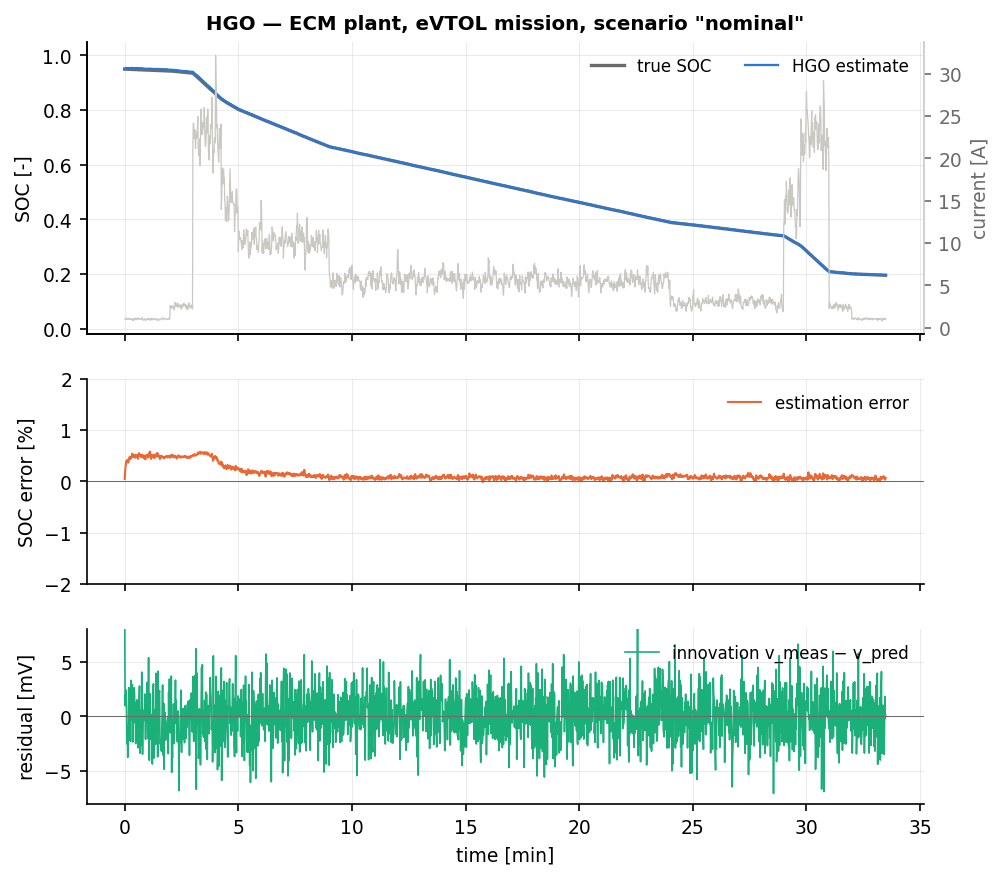
\includegraphics[width=\textwidth]{figures/cell_HGO_nominal.png}
\caption{HGO on the nominal eVTOL mission: true and estimated SOC (top), estimation error with the $\pm 2\sigma$ band when available (middle), voltage residual (bottom).}
\end{figure}
\begin{figure}[H]\centering
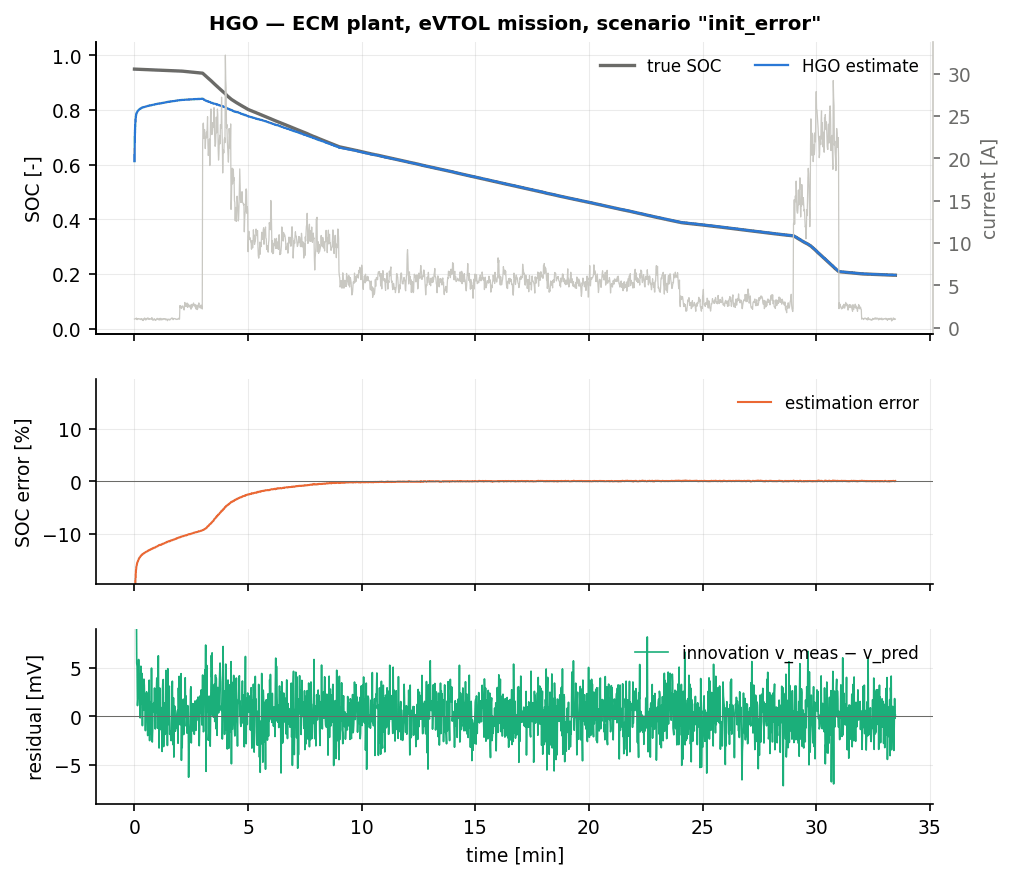
\includegraphics[width=\textwidth]{figures/cell_HGO_init_error.png}
\caption{HGO with a 35\,\% initial SOC error.}
\end{figure}

All numbers are over three seeds.  At the registered setting ($\varepsilon=0.2$,
$\tau_{cl}=60$\,s) the HGO is level with the certified LQE observer on every ECM column:
\texttt{nominal} $\mathrm{rmse}_{ss} = 0.0008$, \texttt{outliers} $0.0017$,
\texttt{sensor\_dropout} $0.0008$, \texttt{noise\_step} $0.0033$, \texttt{cold} $0.0040$,
\texttt{aged\_cell} $0.0218$, \texttt{param\_mismatch} $0.0149$, \texttt{combined} $0.0211$
($0.0204$--$0.0216$ across seeds).  On the single-particle plant it is at $0.0061$
(\texttt{nominal}) and $0.0349$ (\texttt{cold}) against the EKF's $0.0373$ and $0.0735$.

That agreement with \Cref{ch:luenberger} and \Cref{ch:sskf} is itself the finding, and it is a
negative one that this chapter has to state plainly.  The high-gain pole set
$p_i = \exp(-\lambda_i\mu/\varepsilon)$ is a \emph{binomial} set placed by the same Ackermann
machinery, and on this plant that placement almost never passes the certification of
\Cref{sec:lue-schedule}: it is stabilising at the frozen linearisation and unstable under a
$\pm20\,\%$ perturbation of the mode locations or of the OCV slope (\Cref{ch:luenberger} gives the
measured spectral radii).  The observer therefore runs the certified LQE fallback on the great
majority of re-designs, which is why it reproduces the SSKF to four digits.  The anti-peaking
saturation is still active and still doing its job --- it is what keeps the correction bounded
during the \texttt{init\_error} and \texttt{combined} transients --- but the \emph{gain} it
saturates is, most of the time, not a high-gain design.

Where the placement \emph{is} admitted the difference is visible and small: on \texttt{cold} the
HGO and Luenberger agree at $0.0040$ while the pure-LQE SSKF reaches $0.0031$, i.e. the admitted
design is slightly worse than the LQE design it displaced.  On the single-particle plant the one
column where the HGO separates from the LQE observers is \texttt{init\_error} ($0.0186$ against
$0.0259$), where the saturation genuinely earns its place during the $0.35$-SOC transient --- and
it is also the column with the widest seed spread in this chapter ($0.0154$--$0.0235$), because
how long the correction stays saturated depends on the noise realisation.

\section{Summary}
The high-gain observer is the right structure when you want one knob.  Parameterise it as
$\tau_{cl} = \varepsilon/\omega_0$ with binomial nominal roots, place the poles in the original
coordinates with a shifted-and-scaled Ackermann formula rather than forming the canonical
transformation, and always include the Esfandiari--Khalil saturation --- on this plant it is the
difference between a bounded and an unbounded transient.  Expect a lower usable bound on
$\varepsilon$ (here $\approx0.15$) set by the gain budget rather than by theory, and do not expect
small $\varepsilon$ to remove a steady-state bias: for that, estimate the disturbance
(\Cref{ch:dob}) or the parameter (\Cref{ch:adaptiveobserver}).  Most importantly, verify that the
high-gain pole set you asked for is the one you actually got: on a finely sampled plant the
single-output assignment is often not robustly realisable, the certified fallback of
\Cref{sec:lue-schedule} takes over, and an unverified implementation would silently report
high-gain results that are in fact LQE results.
